\documentclass[12pt, a4paper]{article}
\usepackage{../../../myconfig} % Gọi file cấu hình từ ngoài gốc vào

% ==========================================
% BẮT ĐẦU NỘI DUNG TÀI LIỆU
% ==========================================
\begin{document}

% Truyền 3 tham số: {Nhãn cam} {Chữ to chính giữa} {Chữ ở góc phải Header}
\titlebox{Chủ đề: Hàm số}{Tốc độ nước dâng}{Hàm số: Tốc độ nước dâng}

\questionShortAnswer{15}{1}{Một cái bể nước có dạng khối chóp tứ giác đều ngược với cạnh đáy bằng \( 3\sqrt{2} \, dm \) và chiều cao bằng \( 6 \, dm \) (tham khảo hình vẽ bên – các kích thước được nêu ra là phần bên trong hình). Nước được bơm vào bể với tốc độ không đổi là \( 2 \, \text{lít/phút} \) và ban đầu bể không chứa nước (các kết quả bên dưới được làm tròn đến hai chữ số thập phân sau dấu phẩy). Tốc độ dâng lên của nước là bao nhiêu khi thể tích nước trong bể bằng \( \dfrac{1}{3} \) thể tích của bể.
\begin{figure}[htbp]
    
    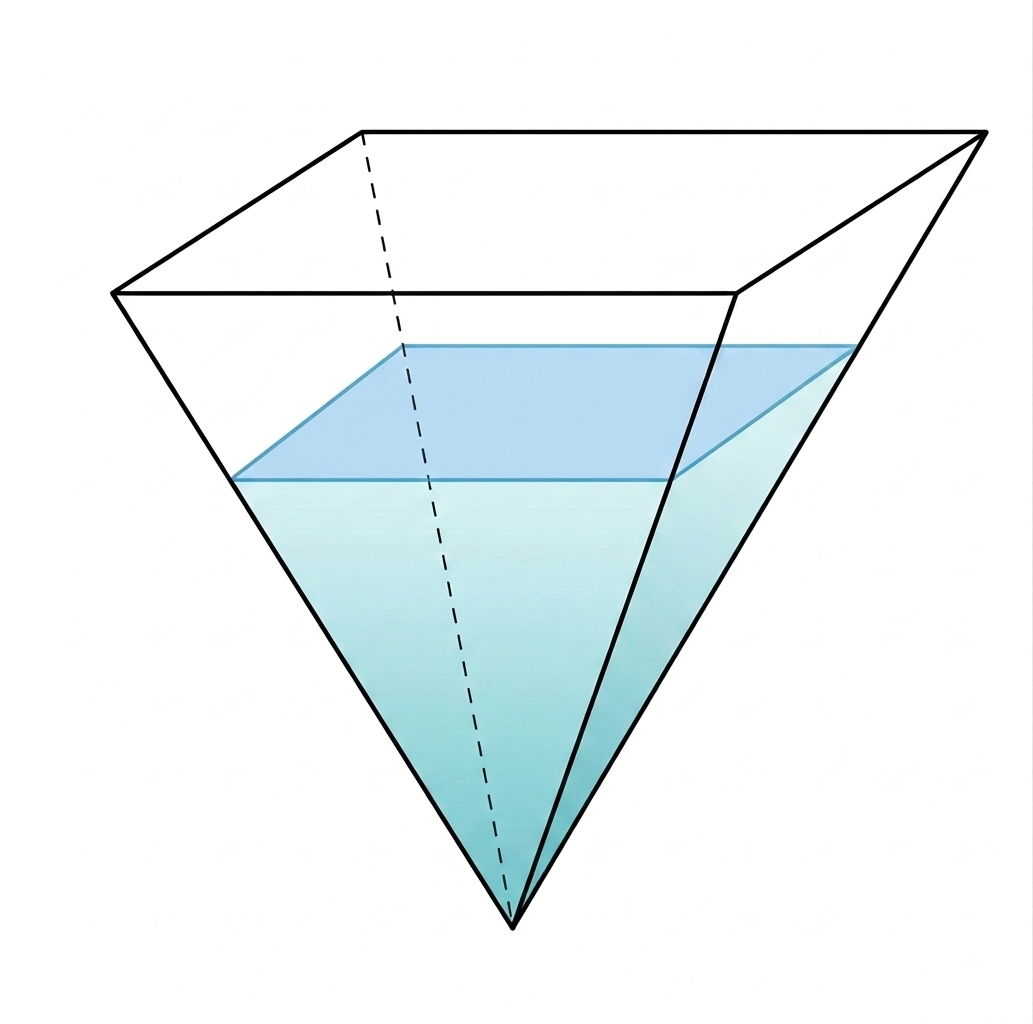
\includegraphics[width=0.3\textwidth]{../images/Hinhchop.png}
    
\end{figure}
}
\newpage
\drawdashlines{33}
\newpage
% --- CÂU 2 ---
\questionShortAnswer{22}{2}{Một cái chậu đựng nước có dạng hình chóp cụt đều, đáy là các tam giác cạnh bằng 1 dm và 3 dm. Chiều cao chậu nước bằng 4 dm. Người ta bơm nước vào chậu với lưu lượng không đổi 0,5 lít/phút đến phút thứ 10, thì tốc độ dâng lên của nước trong chậu là bao nhiêu dm/phút? (Kết quả được làm tròn đến hàng phần trăm).
\begin{figure}[htbp]
    
    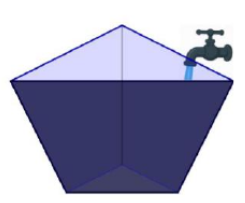
\includegraphics[width=0.3\textwidth]{../images/chopcut3.png}
    
\end{figure}}
\newpage
\drawdashlines{33}
\newpage
% --- CÂU 8 ---
\questionShortAnswer{22}{3}{Một hồ bơi được chế tạo từ một khối hộp chữ nhật có chiều dài 12 mét, rộng 6 mét, sâu 1 mét ở đầu nông và sâu 3 mét ở đầu sâu (như hình vẽ). Nước được bơm vào hồ bơi với tốc độ \( V = 0,25 \, \text{m}^3 \) mỗi phút. Biết rằng trong bể có 1 mét nước ở đầu sâu. Để lượng nước đạt 75\% dung tích bể bơi thì cần bơm trong thời gian bao lâu? (đơn vị tính bằng phút).
\begin{figure}[htbp]
    
    \includegraphics[width=0.4\textwidth]{../images/BeBoi.png}
    
\end{figure}}
\newpage
\drawdashlines{33}
\newpage
% --- CÂU 9 ---
\questionShortAnswer{22}{4}{Thầy T có một cái bể được thiết kế phía dưới là hình hộp chữ nhật có đáy là hình vuông cạnh 10 m, chiều cao là 1 m; phía trên là hình chóp cụt đều có đáy trên là hình vuông cạnh 15 m. Tổng chiều cao của bể là 4 m. Lúc đầu bể không có nước. Thầy T tiến hành bơm nước vào bể với tốc độ không đổi \( 5 \, \text{m}^3/\text{phút} \).  
a) Hỏi tại thời điểm 1 giờ, mực nước trong bể cao bao nhiêu? (đơn vị: m)  
b) Hỏi tại thời điểm 1 giờ 10 phút, tốc độ dâng lên của mực nước trong bể bằng bao nhiêu? (đơn vị: m/phút)
\begin{figure}[htbp]
    
    
\includegraphics[width=0.3\textwidth]{../images/H4.png}
    
\end{figure}}

\newpage
\drawdashlines{33}
\newpage

\end{document}